\section{Method}
\label{sec:method}

\subsection{Preliminaries}

\xhdr{LLM inference} Autoregressive LLM inference involves two stages: \emph{prefill} and \emph{decode}. Prefill encodes the full input to produce the first output token; decode then generates subsequent tokens iteratively using the last token and the cached key–value (KV) states.
Formally, let $X_{[0:n]} = [x_0,\dots,x_{n-1}]$ be the input token sequence. 
After prefill, LLM produces a per-token KV-Cache
$\mathcal{C}(X_{[0:n]}) = [c_0,\dots,c_{n-1}] \in \mathbb{R}^{n \times d}$.
For notation brevity, $d$ denotes the KV dimensionality that is flattened from all layers into a single vector per token.
The range subscripts are omitted when clear.
During decoding, with the current token $y_i$ and caches from the input and the generated prefix, the next token is predicted as
\begin{equation}
    y_{i+1} = \mathcal{P}\!\left(y_i \mid \mathcal{C}(X)\, \oplus\, \mathcal{C}(Y_{[0:i]})\right),
    \label{eq:llm_decode}
\end{equation}
where $\oplus$ denotes sequence-wise concatenation. 
The cache updates as $\mathcal{C}(Y_{[0:i+1]}) = \mathcal{C}(Y_{[0:i]}) \oplus \mathcal{C}(y_i)$.

\xhdr{LLM communication}
In LLM communication scenarios, we define the LLM that provides contextual understanding or knowledge as \emph{Sharer}, and the one that utilizes it as \emph{Receiver}.

\subsection{Oracles for Cache-to-Cache Communication}
\label{sec:oracle}

We aim to explore whether LLMs can have direct semantic communication through KV-Cache.
Specifically, we design two oracle experiments to answer the following questions:
(1) \emph{Benefit}: can a model's capabilities be improved through KV-Cache semantic enrichment without extending sequence length?
(2) \emph{Convertibility}: can the KV-Cache of one model be effectively utilized by another model?

\subsubsection{Cache Enrichment Oracle}
To validate the benefit of cache enrichment, 
we first explore whether the semantic quality of KV-Cache can be improved without increasing its size. 
Few-shot prompting suggests this might work: providing \emph{exemplars} $E$ before the \emph{question} $X$ often improves accuracy. But does this arise from attending to more context tokens, or from $E$ enriching how $X$ is embedded in KV-Cache?

We evaluate this via three setups:
(1) \textit{Direct}: prefill on $X$ only and decode with $\mathcal{C}(X)$;
(2) \textit{Few-shot}: prefill on $E \oplus X$ and decode with $\mathcal{C}(E \oplus X)$ (longer cache);
(3) \textit{Oracle}: prefill on $E \oplus X$ but \emph{discard} the exemplar segment and keep only the question-aligned slice
\begin{equation}
    \mathcal{C}^*(X) \;=\; \mathcal{C}_{[\,|E| : |E|+|X|\,]}(E \oplus X),
    \label{eq:oracle_cache}
\end{equation}
so that decoding uses a question-length cache with no extra tokens. Here, $|\cdot|$ denotes sequence length. In Equation~\ref{eq:llm_decode}, this corresponds to substituting $\mathcal{C}(X)$ with $\mathcal{C}^*(X)$ before decoding.

Comparing \textit{Direct} and \textit{Oracle} isolates the effect of cache enrichment: any gain arises from the richer question embeddings induced by $E$, not from attending to additional token caches as in \textit{Few-shot}. 
As shown in Table~\ref{tab:oracle_left}, the \textit{Oracle} setup improves response quality at the same cache length. 

Additionally, we analyze how cache enrichment affects different transformer layers. 
Our findings show substantial variation across layers: while some layers benefit from cache enrichment, others experience performance degradation (details in Appendix~\ref{sec:appendix/exp/oracle1}). 
Furthermore, these layer-wise effects accumulate as more layers are augmented.
As shown in Figure~\ref{fig:kv_transform_right}, selectively applying cache enrichment to the top-performing layers (e.g., top-5) yields slightly higher accuracy than enriching all layers, while targeting the worst-performing layers leads to accuracy decline. 
This finding guides the gating mechanism of our cache fuser (Section~\ref{sec:method/architecture}).

\begin{figure}[tb]
    \centering
    \begin{minipage}[t]{0.48\textwidth}
        \centering\vspace{0pt}
        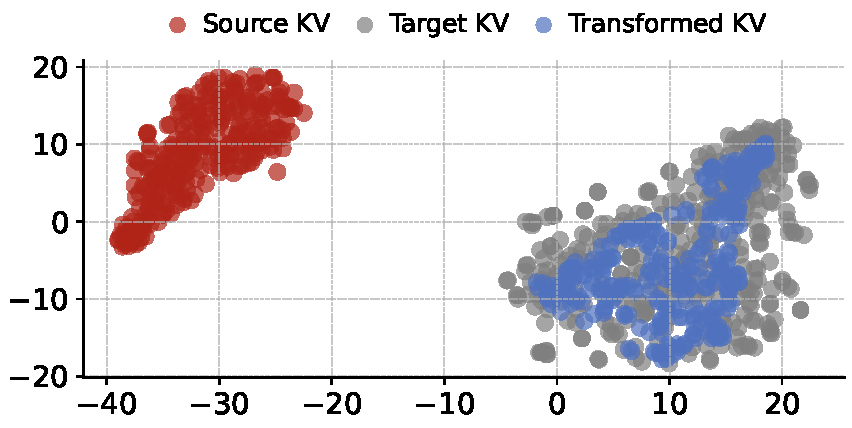
\includegraphics[width=\linewidth]{figure/tsne.pdf}
        \captionof{figure}{T-SNE visualization of KV-Cache representations from the source (Qwen3-4B), target (Qwen3-0.6B), and the transformed cache. After transformation, the source cache falls within the target's representation space.}
        \label{fig:kv_transform_left}
    \end{minipage}
    \hfill
    \begin{minipage}[t]{0.48\textwidth}
        \centering\vspace{0pt}
        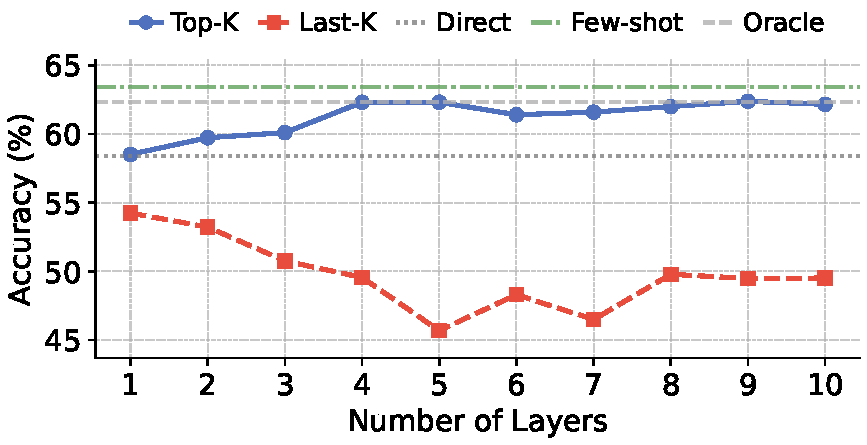
\includegraphics[width=0.99\linewidth]{figure/gate_oracle.pdf}
        \captionof{figure}{Effect of selectively enriching different numbers of layers' KV-Cache on accuracy. Enriching more best-performing layers yields increased accuracy, while enriching the worst-performing ones declines accuracy.}
        \label{fig:kv_transform_right}
    \end{minipage}
\end{figure}

\begin{table}[t]
    \centering
    \begin{minipage}[t]{0.48\textwidth}
        \centering\vspace{4pt}
        \footnotesize
        \setlength\tabcolsep{2pt}
        \begin{tabular}{l|ccc}
        \toprule
        \textbf{Method} & \textbf{Cache Len.} & \textbf{Cache Enrich.} & \textbf{Acc. (\%)} \\
        \midrule
        Direct   & $|X|$        & No  & 58.42\\
        Few-shot & $|E|+|X|$    & Yes & 63.39\\
        Oracle   & $|X|$        & Yes & 62.34\\
        \bottomrule
        \end{tabular}
        \captionof{table}{Cache enrichment experiment. \textit{Oracle} prefills on exemplars ($E$) and question ($X$), then drops the exemplar cache before decoding, isolating semantic enrichment from cache length.}
        \label{tab:oracle_left}
    \end{minipage}
    \hfill
    \begin{minipage}[t]{0.48\textwidth}
        \centering\vspace{0pt}
        \footnotesize
        \setlength\tabcolsep{6pt}
        \begin{tabular}{l|ccc}
        \toprule 
        ~ & \multicolumn{3}{c}{\textbf{Average Effective Rank}} \\
        \cmidrule(lr){2-4}        
        \textbf{Type} & \textbf{Sharer} & \textbf{Receiver} & \textbf{\name} \\
        \midrule
        K Cache   & 539       & 388  & 395\\
        V Cache & 689    & 532 & 560\\
        \bottomrule
        \end{tabular}
        \captionof{table}{Average effective rank of KV-Cache from Sharer, Receiver, and the \name-fused one. The increase after fusion indicates that \name enriches the Receiver KV-Cache semantics.}
        \label{tab:oracle_right}
    \end{minipage}
\end{table}



\subsubsection{Cache Transformation Oracle}
\label{sec:oracle_transform}
To verify that one model's KV-Cache can be utilized by another, we conducted cross-model transformation experiments. 
We train a 3-layer MLP to map the KV-Cache from a source LLM (Qwen3-4B) to a target LLM (Qwen3-0.6B), with more setups detailed in Appendix~\ref{sec:appendix/setup/transformation_oracle}.

T-SNE visualizations in Figure~\ref{fig:kv_transform_left} reveal that the raw KV-Caches of the two LLMs are far apart in representation space. After transformation, the mapped KV-Cache lies inside the target model's representation space. These results demonstrate that KV-Caches from different models are generally convertible, as the transformed cache is covered by the target model's representation space.

One thing to note is that the transformed cache occupies only a smaller subset of the target's space. It indicates that the source model's semantic information cannot fully cover the target's, despite the source being larger. This reflects inherent differences in how each model encodes context. 
Another observation also supports this interpretation: the correct-answer sets of different models exhibit limited overlap (Figure~\ref{fig:venn_breakdown}), despite the comparable aggregated accuracy of respective models. 
These findings suggest that if specialized contextual understanding from different models can be successfully projected and fused, it may harness the complementary strengths of the respective models.

\subsection{\name Design}
\label{sec:C2C}

\subsubsection{Overview}
\label{sec:C2C/scheme}
Building on the oracle experiments, we propose the \name scheme. Its core objective is to extract useful contextual understanding or knowledge from one model (the Sharer) and fuse it into another model (the Receiver). 

In general, the \name paradigm contains a set of key/value cache fusers $\mathcal{F}$ and a layer mapping strategy $\mathcal{G}$. 
During the prefill stage, fuser $\mathcal{F}_{n}$ takes the $n$th layer cache of the Receiver Model $\mathcal{C}_{n}(X)$ and the corresponding $\mathcal{G}(n)$th layer cache of the Sharer Model $\mathcal{C}^{\mathcal{S}}_{\mathcal{G}(n)}(X)$ and generates the corresponding fused cache with residual connection:
\begin{equation}
    \mathcal{C}^{\mathcal{F}} 
    = \left\{
        \mathcal{C}_n(X) +
        \mathcal{F}_{n}\!\left(
            \mathcal{C}_{n}(X),\;
            \mathcal{C}^{\mathcal{S}}_{\mathcal{G}(n)}(X)
        \right)
    \right\}_{n=1}^{N}
\end{equation}


During decoding, with the current token $y_i$ and caches from the input and the generated prefix, the next token is predicted as:

\begin{equation}
y_{i+1} = \mathcal{P}\left( y_i \middle| \mathcal{C}^{\mathcal{F}}(X) \oplus \mathcal{C}(Y_{[0:i]})\right)
\label{eq:llm_decode_clean}
\end{equation}

\begin{figure}[tb]
    \centering
    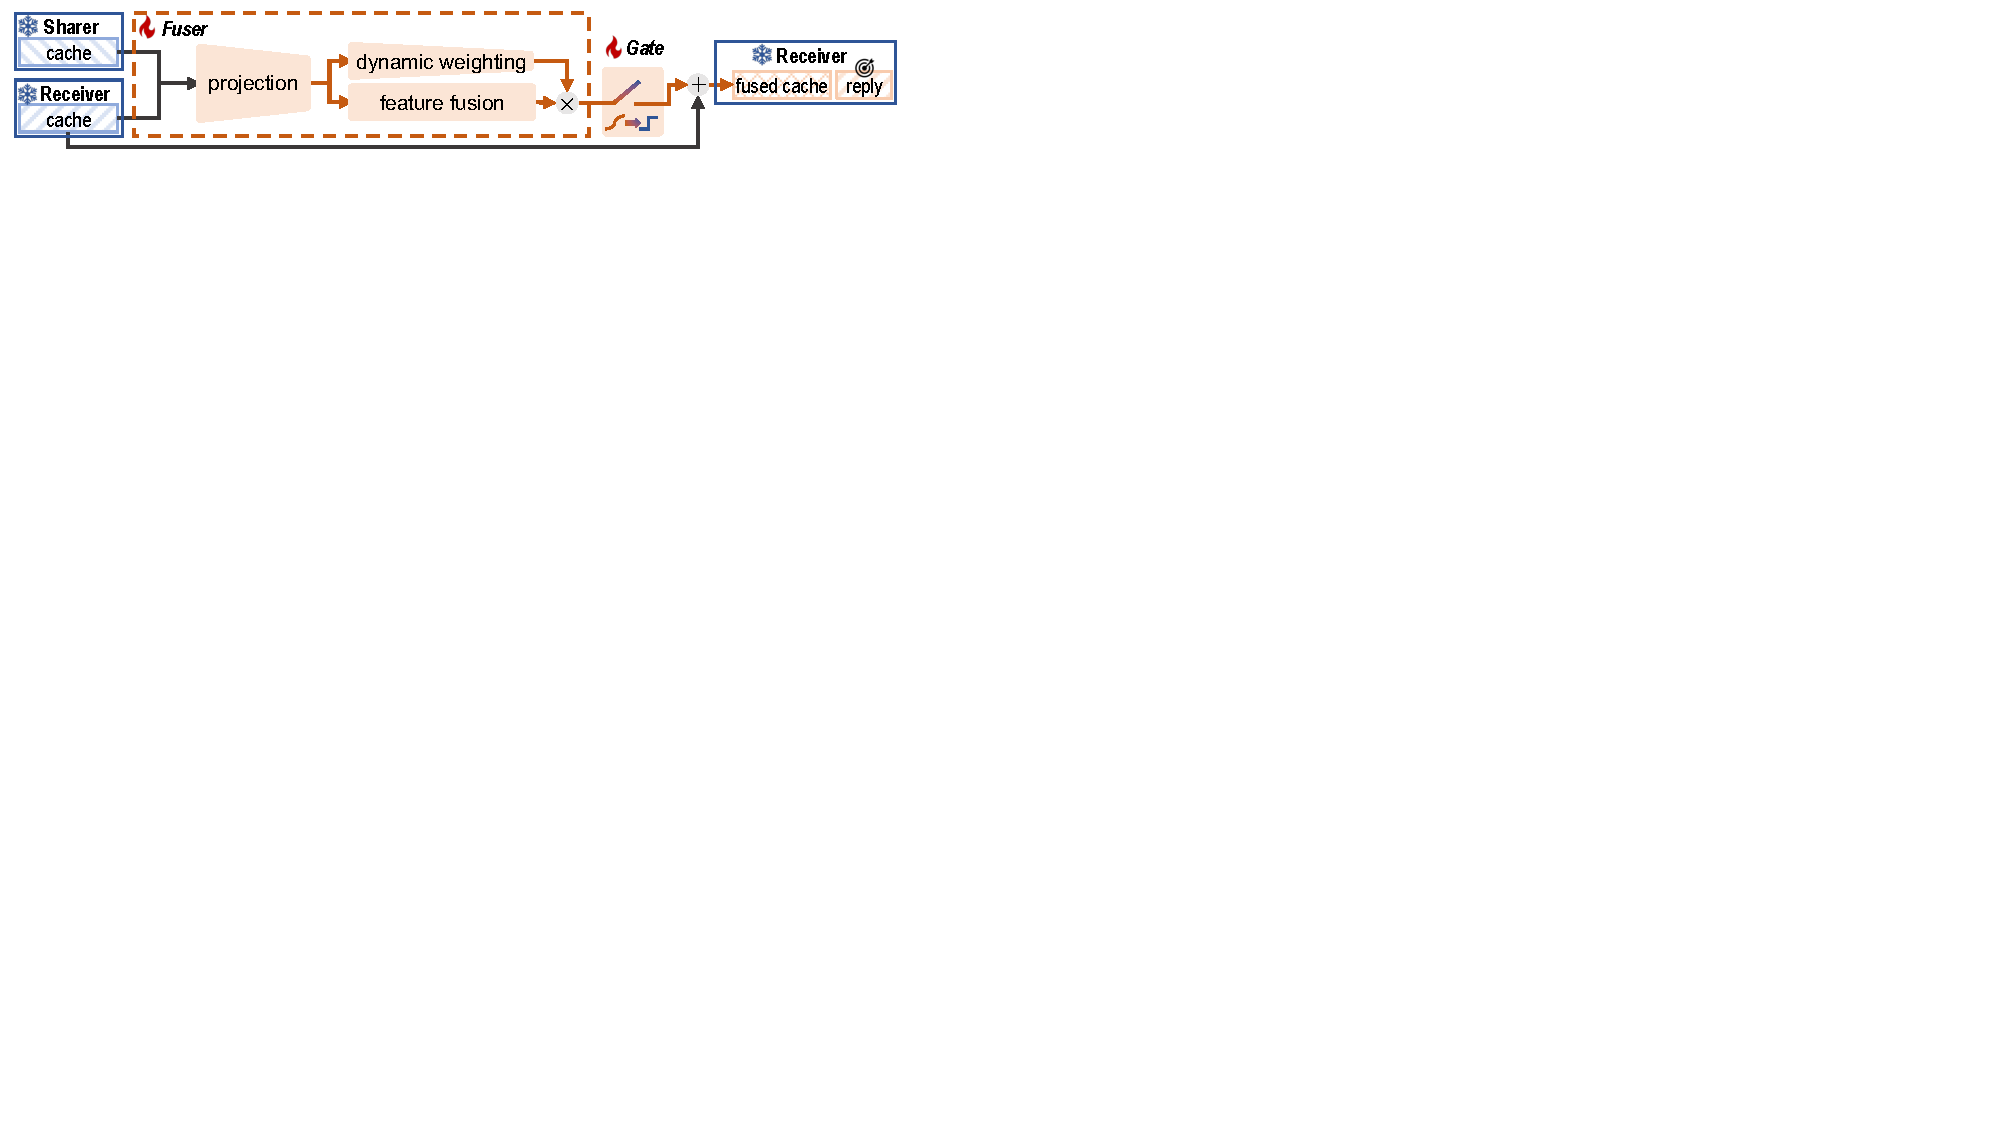
\includegraphics[width=\textwidth]{figure/model_arch.pdf}
    \caption{
        Cache fuser architecture and training scheme. \textit{Fuser} projects and combines KV-Caches, then adds the result to Receiver's cache through a learnable gate. LLMs are frozen during training.
    }
    \label{fig:model_arch}
\end{figure}

\subsubsection{Fuser Structure}
\label{sec:method/architecture}

To enhance the Receiver's KV-Cache without destructive overwriting of its information, the fuser is designed under a residual integration principle. As shown in Figure~\ref{fig:model_arch}, it contains three key modules:

(1) \textbf{Projection module} concatenates the Receiver's KV-Cache with the Sharer's KV-Cache, then processes the concatenated features through a projection layer followed by a feature fusion layer.

(2) \textbf{Dynamic weighting module} applies an input-aware head modulation layer to dynamically reweight the projected information.

(3) \textbf{Learnable gate} introduces a trainable per-layer gate value that decides whether to inject the Sharer's context. The gate applies a Gumbel-sigmoid with temperature annealing to smoothly transition from differentiable during training to binary at inference.

We also explore a more complex yet potentially more powerful fuser variant in Appendix~\ref{sec:appendix/arch}.


\subsubsection{Model Alignment}
Fusing KV-Caches across model families and sizes requires alignment at two levels: tokens and layers.
For \emph{token alignment}, different tokenizers may produce slightly varied token sequences for the same input. 
We align them by decoding each Receiver token into its string form and re-encoding it using the Sharer's tokenizer. 
When one-to-many mappings occasionally occur, we select the Sharer token with maximal string coverage to preserve information.
% layer
For \emph{layer} alignment, we adopt a terminal alignment strategy: the final layers of both models are aligned first, then the penultimate layers, and so on in reverse order until reaching the shallower model's first layer.
Details in Appendices~\ref{sec:appendix/layer_align} and~\ref{sec:appendix/token_align}.

\subsubsection{Training Scheme}

During training, we freeze both the Sharer and Receiver models, training only the \name module for KV-Cache fusion. 
We employ standard next-token prediction loss on the Receiver's response predictions, similar to supervised fine-tuning (SFT). 
The key difference is that the Receiver predicts responses conditioned on fused KV-Cache rather than its own.

The training procedure consists of three stages: 
(1) Forward: both models encode the input context to produce their respective KV-Caches.
(2) Fusion: the \name module fuses both KV-Caches and replaces the Receiver's cache.
(3) Supervision: the Receiver prefills the response using the fused cache, and gradients backpropagate through \name to minimize prediction loss.


